\documentclass[a4paper,10pt]{article}
\usepackage[utf8x]{inputenc}

\usepackage{amsmath}    % need for subequations
\usepackage{graphicx}   % need for figures
\usepackage{verbatim}   % useful for program listings
\usepackage{color}      % use if color is used in text
\usepackage{subfigure}  % use for side-by-side figures
\usepackage{hyperref}   % use for hypertext links, including those to external documents and URLs
\usepackage{cancel} 
\usepackage{titlesec}
\usepackage{array} 	% use for creating arrays such as eqnarray
\setlength{\parskip}{3pt plus 2pt}
\setlength{\parindent}{20pt}

\setlength{\oddsidemargin}{-0.6in}
%\setlength{\evensidemargin}{0.5cm}
%\setlength{\marginparsep}{0.75cm}
%\setlength{\marginparwidth}{2.5cm}
%\setlength{\marginparpush}{1.0cm}
\setlength{\textwidth}{7.4in}
%\headheight{1in}
%\topmargin{0.5in}
%\textheight{10.0in}
%\footheight{0.1in} 


% Colors
\definecolor{headertextcolor}{rgb}{.88,.65,.11}
\definecolor{headerboxcolor}{rgb}{.88,.65,.11}



% Header style
\titleformat{\section}{\color{headertextcolor}\large\scshape\raggedright}{}{0em}{}[\titlerule]
\titleformat{\mbox}{\color{headertextcolor}}{}{}{}

%opening
\title{Maxwell Equations}
\author{Christopher Stricklan}
\date{Revised: February 21, 2011}



\begin{document}

\maketitle

\begin{abstract}
This document describes the reduction from a 3-Dimensional Finite Difference set of Equations as derived in ``Maxwell Equations'' to a 1-Dimensional Form ready for use in numerical modeling algorithms.
\end{abstract}

\vfill



\section{Reduce to One-Dimension}

We will reduce our Finite-Difference Equations to 1D.  This means that we will have material that is uniform in two directions.  
This uniform material will cause the fields to be uniform as well.  The change in material in our case we will define to be in the z-drection therefore the x anx y directions
will be uniform.  This means that the derivates in this direction will also equal zero.

\begin{equation*}
 \frac{\partial}{\partial x} = \frac{\partial}{\partial y}=0
\end{equation*}

\begin{figure}[h]
  \centering
    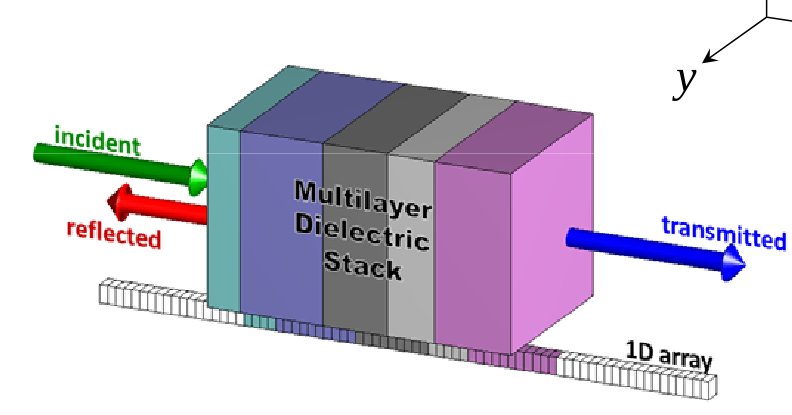
\includegraphics[width=0.5\textwidth]{Slabs1D.png}
  \caption{1D Problem}
\end{figure}


From our Finite-Difference equations we need to cancel out the x and y derivates that are zero.


\begin{equation*}
  \cancel{\frac{\partial E_z}{\partial y}} - \frac{\partial E_y}{\partial z} = -\frac{\mu_{xx}}{c_0}\frac{\partial\tilde{H}_x}{\partial t}
\end{equation*}

\begin{equation*}
  \frac{\partial E_x}{\partial z} - \cancel{\frac{\partial E_z}{\partial x}} = -\frac{\mu_{yy}}{c_0}\frac{\partial\tilde{H}_y}{\partial t}
\end{equation*}

\begin{equation*}
  \cancel{\frac{\partial E_y}{\partial x}} - \cancel{\frac{\partial E_x}{\partial y}} = -\frac{\mu_{zz}}{c_0}\frac{\partial\tilde{H}_z}{\partial t}
\end{equation*}

\begin{equation*}
  \cancel{\frac{\partial \tilde{H}_z}{\partial y}} - \frac{\partial \tilde{H}_y}{\partial z} = \frac{\epsilon_{xx}}{c_0}\frac{\partial E_x}{\partial t}
\end{equation*}

\begin{equation*}
  \frac{\partial \tilde{H}_x}{\partial z} - \cancel{\frac{\partial \tilde{H}_z}{\partial x}} = \frac{\epsilon_{yy}}{c_0}\frac{\partial E_y}{\partial t}
\end{equation*}

\begin{equation*}
  \cancel{\frac{\partial \tilde{H}_y}{\partial x}} - \cancel{\frac{\partial \tilde{H}_x}{\partial y}} = \frac{\epsilon_{zz}}{c_0}\frac{\partial E_z}{\partial t}
\end{equation*}

\[\longrightarrow\]

\begin{equation*}
  \cancel{\frac{E_{z}^{i,j+1,k}\mid_{t} - E_{z}^{i,j,k}\mid_{t}}{\Delta y}} - \frac{E_{y}^{i,j,k+1}\mid_{t} - E_{y}^{i,j,k}\mid_{t}}{\Delta z} = -\frac{\mu_{xx}^{i,j,k}}{c_0} \frac{\tilde{H}_{x}^{i,j,k}\mid_{t+\frac  {\Delta t}{2}} - \tilde{H}_{x}^{i,j,k}\mid_{t-\frac{\Delta t}{2}}}{\Delta t}\notag
\end{equation*}

\begin{equation*}
  \frac{E_{x}^{i,j,k+1}\mid_{t} - E_{x}^{i,j,k}\mid_{t}}{\Delta z} - \cancel{\frac{E_{z}^{i+1,j,k}\mid_{t} - E_{z}^{i,j,k}\mid_{t}}{\Delta x}} = -\frac{\mu_{yy}^{i,j,k}}{c_0} \frac{\tilde{H}_{y}^{i,j,k}\mid_{t+\frac  {\Delta t}{2}} - \tilde{H}_{y}^{i,j,k}\mid_{t-\frac{\Delta t}{2}}}{\Delta t}\notag
\end{equation*}

\begin{equation*}
  \cancel{\frac{E_{y}^{i+1,j,k}\mid_{t} - E_{y}^{i,j,k}\mid_{t}}{\Delta x}} - \cancel{\frac{E_{x}^{i,j+1,k}\mid_{t} - E_{x}^{i,j,k}\mid_{t}}{\Delta y}} = -\frac{\mu_{zz}^{i,j,k}}{c_0} \frac{\tilde{H}_{z}^{i,j,k}\mid_{t+\frac  {\Delta t}{2}} - \tilde{H}_{z}^{i,j,k}\mid_{t-\frac{\Delta t}{2}}}{\Delta t}\notag
\end{equation*}

\begin{equation*}
  \cancel{\frac{\tilde{H}_{z}^{i,j,k}\mid_{t+\frac{\Delta t}{2}} - \tilde{H}_{z}^{i,j-1,k}\mid_{t+\frac  {\Delta t}{2}}}{\Delta y}} - \frac{\tilde{H}_{y}^{i,j,k}\mid_{t+\frac  {\Delta t}{2}} - \tilde{H}_{y}^{i,j,k-1}\mid_{t+\frac  {\Delta t}{2}}}{\Delta z} = \frac{\epsilon_{xx}^{i,j,k}}{c_0} \frac{E_{x}^{i,j,k}\mid_{t+\Delta t} - E_{x}^{i,j,k}\mid_{t}}{\Delta t}\notag
\end{equation*}

\begin{equation*}
  \frac{\tilde{H}_{x}^{i,j,k}\mid_{t+\frac{\Delta t}{2}} - \tilde{H}_{x}^{i,j,k-1}\mid_{t+\frac  {\Delta t}{2}}}{\Delta z} - \cancel{\frac{\tilde{H}_{z}^{i,j,k}\mid_{t+\frac  {\Delta t}{2}} - \tilde{H}_{z}^{i-1,j,k}\mid_{t+\frac  {\Delta t}{2}}}{\Delta x}} = \frac{\epsilon_{yy}^{i,j,k}}{c_0} \frac{E_{y}^{i,j,k}\mid_{t+\Delta t} - E_{y}^{i,j,k}\mid_{t}}{\Delta t}\notag
\end{equation*}

\begin{equation*}
  \cancel{\frac{\tilde{H}_{y}^{i,j,k}\mid_{t+\frac{\Delta t}{2}} - \tilde{H}_{y}^{i-1,j,k}\mid_{t+\frac  {\Delta t}{2}}}{\Delta x}} - \cancel{\frac{\tilde{H}_{x}^{i,j,k}\mid_{t+\frac  {\Delta t}{2}} - \tilde{H}_{x}^{i,j-1,k}\mid_{t+\frac  {\Delta t}{2}}}{\Delta y}} = \frac{\epsilon_{zz}^{i,j,k}}{c_0} \frac{E_{z}^{i,j,k}\mid_{t+\Delta t} - E_{z}^{i,j,k}\mid_{t}}{\Delta t}\notag
\end{equation*}


With these cross outs we come out with two observations.  The first is that the longitudinal field components Ez and Hz are always zero.  The second is that the Maxwell's equations have decoupled into two sets of two equations Ex/Hy Mode and Ey/Hx Mode.

\begin{equation*}
  - \frac{\partial E_y}{\partial z} = -\frac{\mu_{xx}}{c_0}\frac{\partial\tilde{H}_x}{\partial t}
\end{equation*}

\begin{equation*}
  \frac{\partial E_x}{\partial z} = -\frac{\mu_{yy}}{c_0}\frac{\partial\tilde{H}_y}{\partial t}
\end{equation*}

\begin{equation*}
  0 = -\frac{\mu_{zz}}{c_0}\frac{\partial\tilde{H}_z}{\partial t}
\end{equation*}

\begin{equation*}
  - \frac{\partial \tilde{H}_y}{\partial z} = \frac{\epsilon_{xx}}{c_0}\frac{\partial E_x}{\partial t}
\end{equation*}

\begin{equation*}
  \frac{\partial \tilde{H}_x}{\partial z} = \frac{\epsilon_{yy}}{c_0}\frac{\partial E_y}{\partial t}
\end{equation*}

\begin{equation*}
  0 = \frac{\epsilon_{zz}}{c_0}\frac{\partial E_z}{\partial t}
\end{equation*}

\[\longrightarrow\]

\begin{equation*}
  - \frac{E_{y}^{i,j,k+1}\mid_{t} - E_{y}^{i,j,k}\mid_{t}}{\Delta z} = -\frac{\mu_{xx}^{i,j,k}}{c_0} \frac{\tilde{H}_{x}^{i,j,k}\mid_{t+\frac  {\Delta t}{2}} - \tilde{H}_{x}^{i,j,k}\mid_{t-\frac{\Delta t}{2}}}{\Delta t}\notag
\end{equation*}

\begin{equation*}
  \frac{E_{x}^{i,j,k+1}\mid_{t} - E_{x}^{i,j,k}\mid_{t}}{\Delta z} = -\frac{\mu_{yy}^{i,j,k}}{c_0} \frac{\tilde{H}_{y}^{i,j,k}\mid_{t+\frac  {\Delta t}{2}} - \tilde{H}_{y}^{i,j,k}\mid_{t-\frac{\Delta t}{2}}}{\Delta t}\notag
\end{equation*}

\begin{equation*}
  \tilde{H}_{z}^{i,j,k} = 0\notag
\end{equation*}

\begin{equation*}
  - \frac{\tilde{H}_{y}^{i,j,k}\mid_{t+\frac  {\Delta t}{2}} - \tilde{H}_{y}^{i,j,k-1}\mid_{t+\frac  {\Delta t}{2}}}{\Delta z} = \frac{\epsilon_{xx}^{i,j,k}}{c_0} \frac{E_{x}^{i,j,k}\mid_{t+\Delta t} - E_{x}^{i,j,k}\mid_{t}}{\Delta t}\notag
\end{equation*}

\begin{equation*}
  \frac{\tilde{H}_{x}^{i,j,k}\mid_{t+\frac{\Delta t}{2}} - \tilde{H}_{x}^{i,j,k-1}\mid_{t+\frac  {\Delta t}{2}}}{\Delta z} = \frac{\epsilon_{yy}^{i,j,k}}{c_0} \frac{E_{y}^{i,j,k}\mid_{t+\Delta t} - E_{y}^{i,j,k}\mid_{t}}{\Delta t}\notag
\end{equation*}

\begin{equation*}
  E_{z}^{i,j,k} = 0\notag
\end{equation*}


\section{Summary of 1D Finite-Difference Equations}

The equations are now broken apart into their respective modes.  These modes are physical and propage independently from each other.  In the end though they are numerically the same and will exhibit the same electromagnetic behavior.   This allows us to only have to solve one set of two equations.  We can also note that since we only changing materials along the z axis we can drop the i and j Array Indices.



\textbf{Ex/Hy Mode}
\begin{equation}
  - \frac{\tilde{H}_{y}^{k}\mid_{t+\frac  {\Delta t}{2}} - \tilde{H}_{y}^{k-1}\mid_{t+\frac  {\Delta t}{2}}}{\Delta z} = \frac{\epsilon_{xx}^{k}}{c_0} \frac{E_{x}^{k}\mid_{t+\Delta t} - E_{x}^{k}\mid_{t}}{\Delta t}
\end{equation}

\begin{equation}
  \frac{E_{x}^{k+1}\mid_{t} - E_{x}^{k}\mid_{t}}{\Delta z} = -\frac{\mu_{yy}^{k}}{c_0} \frac{\tilde{H}_{y}^{k}\mid_{t+\frac  {\Delta t}{2}} - \tilde{H}_{y}^{k}\mid_{t-\frac{\Delta t}{2}}}{\Delta t}
\end{equation}



\textbf{Ey/Hx Mode}
\begin{equation}
  \label{eq:EinEyHXMode}
  \frac{\tilde{H}_{x}^{k}\mid_{t+\frac{\Delta t}{2}} - \tilde{H}_{x}^{k-1}\mid_{t+\frac  {\Delta t}{2}}}{\Delta z} = \frac{\epsilon_{yy}^{k}}{c_0} \frac{E_{y}^{k}\mid_{t+\Delta t} - E_{y}^{k}\mid_{t}}{\Delta t}
\end{equation}

\begin{equation}
  \label{eq:HinEyHxMode}
  \frac{E_{y}^{k+1}\mid_{t} - E_{y}^{k}\mid_{t}}{\Delta z} = \frac{\mu_{xx}^{k}}{c_0} \frac{\tilde{H}_{x}^{k}\mid_{t+\frac  {\Delta t}{2}} - \tilde{H}_{x}^{k}\mid_{t-\frac{\Delta t}{2}}}{\Delta t}
\end{equation}


\section{Update Equations}
We are now going to derive the update equations used during in FDTD algorithm.  We have arbitrarily chosen to use Ey/Hx Mode found in Equations \eqref{eq:EinEyHXMode} and \eqref{eq:HinEyHxMode}

Update Equation for Ey

\begin{equation*}
  \frac{\tilde{H}_{x}^{k}\mid_{t+\frac{\Delta t}{2}} - \tilde{H}_{x}^{k-1}\mid_{t+\frac  {\Delta t}{2}}}{\Delta z} = \frac{\epsilon_{yy}^{k}}{c_0} \frac{E_{y}^{k}\mid_{t+\Delta t} - E_{y}^{k}\mid_{t}}{\Delta t}
\end{equation*}

We want to solve for the E-Field at the future time value.

\begin{equation*}
  \frac{\epsilon_{yy}^{k}}{c_0} \frac{E_{y}^{k}\mid_{t+\Delta t} - E_{y}^{k}\mid_{t}}{\Delta t} = \frac{\tilde{H}_{x}^{k}\mid_{t+\frac{\Delta t}{2}} - \tilde{H}_{x}^{k-1}\mid_{t+\frac  {\Delta t}{2}}}{\Delta z}
\end{equation*}

\begin{equation*}
  E_{y}^{k}\mid_{t+\Delta t} - E_{y}^{k}\mid_{t} = \frac{c_0\Delta t}{\epsilon_{yy}^{k}} \left(\frac{\tilde{H}_{x}^{k}\mid_{t+\frac{\Delta t}{2}} - \tilde{H}_{x}^{k-1}\mid_{t+\frac  {\Delta t}{2}}}{\Delta z}\right)
\end{equation*}

\begin{equation}
  E_{y}^{k}\mid_{t+\Delta t} = E_{y}^{k}\mid_{t} + \left(\frac{c_0\Delta t}{\epsilon_{yy}^{k}}\right) \left( \frac{\tilde{H}_{x}^{k}\mid_{t+\frac{\Delta t}{2}} - \tilde{H}_{x}^{k-1}\mid_{t+\frac  {\Delta t}{2}}}{\Delta z}\right)
\end{equation}


Update Equation for Hx

\begin{equation*}
  \frac{E_{y}^{k+1}\mid_{t} - E_{y}^{k}\mid_{t}}{\Delta z} = \frac{\mu_{xx}^{k}}{c_0} \frac{\tilde{H}_{x}^{k}\mid_{t+\frac  {\Delta t}{2}} - \tilde{H}_{x}^{k}\mid_{t-\frac{\Delta t}{2}}}{\Delta t}
\end{equation*}

We want to sove for the H-Field at the future time value

\begin{equation*}
  \frac{\mu_{xx}^{k}}{c_0} \frac{\tilde{H}_{x}^{k}\mid_{t+\frac  {\Delta t}{2}} - \tilde{H}_{x}^{k}\mid_{t-\frac{\Delta t}{2}}}{\Delta t} = \frac{E_{y}^{k+1}\mid_{t} - E_{y}^{k}\mid_{t}}{\Delta z}
\end{equation*}

\begin{equation*}
  \tilde{H}_{x}^{k}\mid_{t+\frac{\Delta t}{2}} - \tilde{H}_{x}^{k}\mid_{t-\frac{\Delta t}{2}} = \frac{c_0\Delta t}{\mu_{xx}^{k}}\left(\frac{E_{y}^{k+1}\mid_{t} - E_{y}^{k}\mid_{t}}{\Delta z}\right)
\end{equation*}

\begin{equation}
  \tilde{H}_{x}^{k}\mid_{t+\frac{\Delta t}{2}} = \tilde{H}_{x}^{k}\mid_{t-\frac{\Delta t}{2}} + \left(\frac{c_0\Delta t}{\mu_{xx}^{k}}\right)\left(\frac{E_{y}^{k+1}\mid_{t} - E_{y}^{k}\mid_{t}}{\Delta z}\right)
\end{equation}

\section{Update Coefficients}

Since the update coefficients don't change during the simulation.  We can compute them once before our FDTD Algorithm is actually implemented in loop.

\begin{equation}
  \tilde{H}_{x}^{k}\mid_{t+\frac{\Delta t}{2}} = \tilde{H}_{x}^{k}\mid_{t-\frac{\Delta t}{2}} + m_{H_x}^{k}\left(\frac{E_{y}^{k+1}\mid_{t} - E_{y}^{k}\mid_{t}}{\Delta z}\right)
\end{equation}

\begin{equation}
  E_{y}^{k}\mid_{t+\Delta t} = E_{y}^{k}\mid_{t} + m_{E_y}^{k}\left(\frac{\tilde{H}_{x}^{k}\mid_{t+\frac{\Delta t}{2}} - \tilde{H}_{x}^{k-1}\mid_{t+\frac  {\Delta t}{2}}}{\Delta z}\right)
\end{equation}


\begin{equation}
  m_{E_y}^{k} = \frac{c_0 \Delta t}{\epsilon_{yy}^{k}}
\end{equation}

\begin{equation}
   m_{H_x}^{k} = \frac{c_0 \Delta t}{\mu_{yy}^{k}}
\end{equation}



\section{Boundary Conditions}
We have two types of boundary conditions that can be incorporated into this 1-Dimensional Simulation.  The Dirichlet and Perfectly Absorbing Boundary Conditions are methods that allow us to handle the fields that lie at the boundary of the model.  Specifically these points lie at $k = 0$ and $k = N_z+1$.  At these points there is no grid to pull our Electric and Magnetic fields from, therefore to maintain the stability of the Finite Difference Maxwell's Equations we must handle these seperatly.

\textbf{Dirichlet Boundary Condition}
This boundary condition is the easiest to implement.  We simply assume the fields that lie outside the grid are zero.  This is the most crude method and will cause reflection back into our model as energy reaches the boundary.


\begin{eqnarray*}
  \mbox{For } k < N_z & \tilde{H}_{x}^{k}\mid_{t+\frac{\Delta t}{2}} = \tilde{H}_{x}^{k}\mid_{t-\frac{\Delta t}{2}} + m_{H_x}^{k}\left(\frac{E_{y}^{k+1}\mid_{t} - E_{y}^{k}\mid_{t}}{\Delta z}\right) \\
  \mbox{For } k = N_z & \tilde{H}_{x}^{k}\mid_{t+\frac{\Delta t}{2}} = \tilde{H}_{x}^{k}\mid_{t-\frac{\Delta t}{2}} + m_{H_x}^{k}\left(\frac{0 - E_{y}^{k}\mid_{t}}{\Delta z}\right)
\end{eqnarray*}



\begin{eqnarray*}
  \mbox{For } k > 1 & E_{y}^{k}\mid_{t+\Delta t} = E_{y}^{k}\mid_{t} + m_{E_y}^{k}\left(\frac{\tilde{H}_{x}^{k}\mid_{t+\frac{\Delta t}{2}} - \tilde{H}_{x}^{k-1}\mid_{t+\frac  {\Delta t}{2}}}{\Delta z}\right)\\
  \mbox{For } k = 1 & E_{y}^{k}\mid_{t+\Delta t} = E_{y}^{k}\mid_{t} + m_{E_y}^{k}\left(\frac{\tilde{H}_{x}^{k}\mid_{t+\frac{\Delta t}{2}} - 0}{\Delta z}\right)
\end{eqnarray*}

\textbf{Periodic Boundary Condition}
This boundary condition assumes that the device being modeled is periodic along a particular direction.  In our case the periodicity is along the z-axis. 

\begin{eqnarray*}
  \mbox{For } k < N_z & \tilde{H}_{x}^{k}\mid_{t+\frac{\Delta t}{2}} = \tilde{H}_{x}^{k}\mid_{t-\frac{\Delta t}{2}} + m_{H_x}^{k}\left(\frac{E_{y}^{k+1}\mid_{t} - E_{y}^{k}\mid_{t}}{\Delta z}\right)\\
  \mbox{For } k = N_z & \tilde{H}_{x}^{k}\mid_{t+\frac{\Delta t}{2}} = \tilde{H}_{x}^{k}\mid_{t-\frac{\Delta t}{2}} + m_{H_x}^{k}\left(\frac{E_{y}^{1}\mid_{t} - E_{y}^{N_z}\mid_{t}}{\Delta z}\right)
\end{eqnarray*}

\begin{eqnarray*}
  \mbox{For } k > 1 & E_{y}^{k}\mid_{t+\Delta t} = E_{y}^{k}\mid_{t} + m_{E_y}^{k}\left(\frac{\tilde{H}_{x}^{k}\mid_{t+\frac{\Delta t}{2}} - \tilde{H}_{x}^{k-1}\mid_{t+\frac  {\Delta t}{2}}}{\Delta z}\right)\\
  \mbox{For } k = 1 & E_{y}^{k}\mid_{t+\Delta t} = E_{y}^{k}\mid_{t} + m_{E_y}^{k}\left(\frac{\tilde{H}_{x}^{1}\mid_{t+\frac{\Delta t}{2}} - \tilde{H}_{x}^{N_z}\mid_{t+\frac  {\Delta t}{2}}}{\Delta z}\right)
\end{eqnarray*}


\textbf{Perfectly Absorbing Boundary Condition}
The Perfectly Absorbing Boundary Condition provides a method to absorb almost all of the energy out of the model.  There is approximately 10 orders of magnitude less energy reflected back into the problem space.  This is very minor and should not affect our results.  There are three conditions though that must be met in order to use this boundary conditionl.
\begin{itemize}
\item Waves at the boundaries are only traveling outward.
\item Materials at the boundaries are linear, homogeneous, isotropic and non-dispersive.
\item Time step is chosen so physical waves travel 1 cell in two time steps $\Delta t=\frac{\Delta z}{2c_o}$
\end{itemize}

\begin{figure}[ht]
  \label{fig:PerfectBoundary}
   \centering
     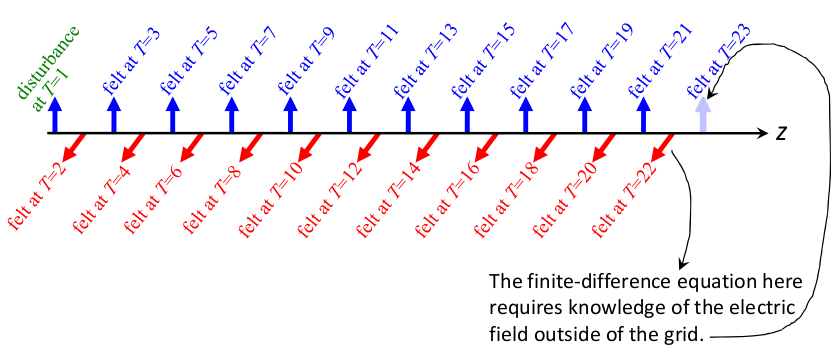
\includegraphics[width=0.75\textwidth]{PerfectBoundary.png}
   \caption{Perfeect Boundary Time Steps}
\end{figure}

As can be seen in \ref{fig:PerfectBoundary} the last time step is magically off the grid.  In order to implement the perfect boundary condition we must use a field that would have propagated past our last grid cell $2\Delta t$ time steps ago.   In equations \eqref{eq:PerfectboundaryH} and \eqref{eq:PerfectboundaryE} the field value that exists outside our cells needs to be used when the wave reaches it at the $2\Delta t$ time frame

\begin{equation}
  \label{eq:PerfectboundaryH}
  \tilde{H}_{x}^{k}\mid_{t+\frac{\Delta t}{2}} = \tilde{H}_{x}^{k}\mid_{t-\frac{\Delta t}{2}} + m_{H_x}^{k}\left(\frac{E_{y}^{N_z+1}\mid_{t} - E_{y}^{N_z}\mid_{t}}{\Delta z}\right)
\end{equation}

\begin{equation}
  \label{eq:PerfectboundaryE}
  E_{y}^{k}\mid_{t+\Delta t} = E_{y}^{k}\mid_{t} + m_{E_y}^{k}\left(\frac{\tilde{H}_{x}^{1}\mid_{t+\frac{\Delta t}{2}} - \tilde{H}_{x}^{0}\mid_{t+\frac  {\Delta t}{2}}}{\Delta z}\right)
\end{equation}

Since the field values did exist $2\Delta t$ ago in our boundary cell in the problem space.  We can then infer the value is the same as the energy leaves the grid.

\begin{equation*}
  E_y^{N_z + 2}\mid_{t} = E_y^{N_z}\mid_{t-2\Delta t}
\end{equation*}

\begin{equation*}
 \tilde{H}_{x}^{0}\mid_{t} = \tilde{H}_{x}^{1}\mid_{t-2\Delta t}
\end{equation*}

To implement the boundary condition we keep track of previous history in variables.  At the z-low boundary we only modify the E-Field update equations.  At the z-high boundary we only modify the H-Field update equations.


\begin{eqnarray*}
  h_3 = h_2 & h_2 = h_1 & h1 = \tilde{H}_{x}^{1}\\
\end{eqnarray*}

\begin{equation*}
   E_{y}^{k}\mid_{t+\Delta t} = E_{y}^{1}\mid_{t} + m_{E_y}^{1}\left(\frac{\tilde{H}_{x}^{1}\mid_{t+\frac{\Delta t}{2}} - h_3 }{\Delta z}\right)
\end{equation*}


\begin{eqnarray*}
  e_3 = e_2 & e_2 = e_1 & e_1 = E_y^{N_z}\\
\end{eqnarray*}

\begin{equation*}
   \tilde{H}_{x}^{N_z}\mid_{t+\frac{\Delta t}{2}} = \tilde{H}_{x}^{N_z}\mid_{t-\frac{\Delta t}{2}} + m_{H_x}^{N_z}\left(\frac{e_3 - E_{y}^{N_z}\mid_{t}}{\Delta z}\right)\\
\end{equation*}


\end{document}
